% Creating a simple Title Page in Beamer
\documentclass{beamer}

% Theme choice:
\usetheme{AnnArbor}

% customize the caption
\setbeamerfont{caption}{size=\large}
\setbeamercolor{caption}{fg=blue}
\setbeamercolor{caption name}{fg=red}

% Title page details:
\title{Introduction to Topology}
\author{yuzuki}
\institute{Eyes, Japan}
\date{\today}
\logo{

\includegraphics[width=3cm]{eyes-japan-logo.png}
}

\begin{document}

% Title page frame
\begin{frame}
    \titlepage
\end{frame}

% Outline frame
\begin{frame}{Outline}
    \tableofcontents
\end{frame}

% Current section
\AtBeginSection[ ]
{
\begin{frame}{Outline}
    \tableofcontents[currentsection]
\end{frame}
}

% Presentation structure
\section{Euler's theorem}

\begin{frame}{Euler's theorem}
\begin{columns}
% Column 1
\begin{column}{0.5\textwidth}
        Here I can explain in detail what the figure represents.
\end{column}
% Column 2
\begin{column}{0.5\textwidth}
    \begin{figure}
    \centering
        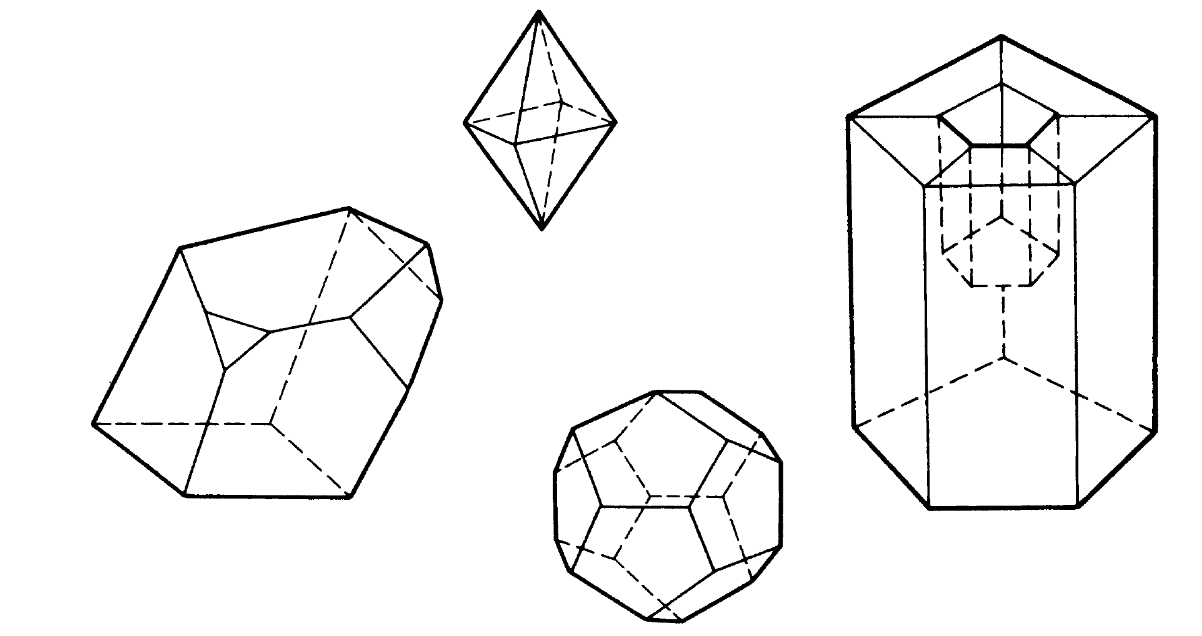
\includegraphics[width=0.7\textwidth]{figure_1_1.png}
        \caption{A figure that is next to a certain explanation.}
    \end{figure}
\end{column}
\end{columns}
\end{frame}

\section{Topological equivalence}
    \subsection{v - e + f = 2}
    \subsection{v - e + f = 4}
    \subsection{v - e + f = 0}
    \subsection{Outline proof of Euler's theorem}
\section{Surfaces}
\section{Abstract spaces}
\section{A classification theorem}

\end{document}